\documentclass[table]{beamer}
\usepackage{graphicx}
\usepackage{color}
\usepackage{pgfpages}
\usepackage{amsmath}
\usepackage{booktabs}
\usepackage{listings}
\usepackage{graphicx}
\usepackage{multirow}

\makeatother
\setbeamertemplate{footline}
{
  % \leavevmode%
  % \hbox{%
  % \begin{beamercolorbox}[wd=.4\paperwidth,ht=2.25ex,dp=1ex,center]{author in head/foot}%
  %   \usebeamerfont{author in head/foot}\insertshortauthor
  % \end{beamercolorbox}%
  % \begin{beamercolorbox}[wd=.6\paperwidth,ht=2.25ex,dp=1ex,center]{title in head/foot}%
  %   \usebeamerfont{title in head/foot}\insertshorttitle\hspace*{3em}
  %   \insertframenumber{} / \inserttotalframenumber\hspace*{1ex}
  % \end{beamercolorbox}}%
  % \vskip0pt%
}
\makeatletter

\setbeamertemplate{footline}[page number]{}

\setbeamertemplate{navigation symbols}{}

\definecolor{mygray}{rgb}{0.9,0.9,0.9}

\lstset{
    basicstyle=\footnotesize\ttfamily,
    tabsize=2,
    backgroundcolor=\color{mygray},
    escapeinside={(*}{*)}
}

% \usetheme{Malmoe} 
\usetheme{Szeged} 
\usecolortheme{beaver}

% Remove nav buttons
% \beamertemplatenavigationsymbolsempty
\setbeamercolor{navigation symbols}{fg=black, bg=white}



\title{Safety $\neq$ Security}
\subtitle{A SECURITY EVALUATION OF STATE OF THE ART AUTOMOTIVE MICROCONTROLLERS}
\date{May 2, 2017}
\author{Nils Wiersma}

\titlegraphic{\includegraphics[width=3cm]{../../pics/riscurelogo.png}% \hspace{5cm}% \ \\%
  \hspace{1cm}  
 \includegraphics[width=5cm]{../../pics/rulogo.pdf}
}


\usepackage{cleveref}

\usepackage{import}
\graphicspath{{pics/}{../../pics/}}

\begin{document}

\begin{frame}
    \titlepage
\end{frame}

\begin{frame}
    \tableofcontents
\end{frame}

\section{Introduction}

\begin{frame}
    \tableofcontents[currentsection]
\end{frame}


\begin{frame}{Riscure}
    What do they do?
    \begin{itemize}
        \item Security evaluation, including SCA and FI
        \item Security training, including SCA and FI
        \item Make tools for SCA and FI
        \item Research
    \end{itemize}
\end{frame}

\begin{frame}{Riscure}
    What did they do for me?
    \begin{itemize}
        \item Initial topic
        \item Ramiro and Albert
        \item Equipment and workspace
    \end{itemize}
\end{frame}

\begin{frame}{Topic}
    \begin{itemize}
        \item Investigate the security of modern microcontroller units, 
            \item[] used in the automotive industry, 
            \item[] by means of fault injection.
    \end{itemize}

\end{frame}

\begin{frame}{Why fault injection?}
    \begin{itemize}
        \item Increased security on certain fronts
        \item Other roads of exploitation
    \end{itemize}
\end{frame}

\begin{frame}{Why the automotive microcontrollers?}
    
    \begin{itemize}
        \item Harsh environment
        \item Safety critical
        \item Fault tolerant
        \item ISO26262
        \item Safety mechanisms
        % \item Mass production 
    \end{itemize}
\end{frame}

\begin{frame}{Why the automotive microcontrollers?}
    \begin{itemize}
        \item Safety mechanisms as countermeasures
        \item Mass production
    \end{itemize}
\end{frame}

\section{Fault Injection}

\begin{frame}
    \tableofcontents[currentsection]
\end{frame}

\begin{frame}{Fault injection}
    \begin{itemize}
        \item Inject glitch in the environment
        \item Produce useful fault
    \end{itemize}
\end{frame}

\begin{frame}{Fault injection}
    \begin{itemize}
        \item Clock 
        \item Optical 
        % \item Temperature
    \end{itemize}
    \ \\
    \begin{itemize}
        \item Power
        \item Electromagnetic
    \end{itemize}
\end{frame}

\begin{frame}{Fault injection}
    \begin{figure}[H]
    \centering
    \def\svgwidth{\columnwidth}
    \input{../../pics/FIdiagram-icWaves.pdf_tex}
    \end{figure}
\end{frame}

\begin{frame}{Fault injection}
    \begin{figure}[H]
    \centering
    \def\svgwidth{\columnwidth}
    \input{../../pics/FIdiagram-EM.pdf_tex}
    \end{figure}
\end{frame}

\begin{frame}{Fault injection}
    \begin{figure}[H]
      \centering
      \includegraphics[width=\textwidth]{../../pics/photos/setup-clean-1.jpg}
    \end{figure}
\end{frame}

\begin{frame}{Fault injection}
    \begin{figure}[H]
      \centering
      \includegraphics[width=\textwidth]{../../pics/photos/setup-messy-1.jpg}
    \end{figure}
\end{frame}

\begin{frame}{Fault injection}
    \begin{figure}[H]
      \centering
      \includegraphics[width=\textwidth]{../../pics/photos/IMG_20170119_164107-1.jpg}
    \end{figure}
\end{frame}


\begin{frame}{Fault injection}
    \begin{figure}[H]
      \centering
      \includegraphics[width=\textwidth]{../../pics/photos/IMG_20161229_145504-1.jpg}
    \end{figure}
\end{frame}

\begin{frame}{Fault injection}
    \begin{itemize}
        \item Flip bits
    \end{itemize}
\end{frame}

% \begin{frame}{Fault injection}
%     \begin{table}[H]
%           \begin{tabular}{l r}
%         01010101 &
%         85 \\
%         0\textbf{0}010101 &
%         21  \\
%           \end{tabular}
%     \end{table}
% \end{frame}

\begin{frame}{Fault injection}
    int flag = 1; \\
    if (flag == 0) \\
    \     bad(); \\
    else \\
    \     good(); 
\end{frame}

\begin{frame}{Fault injection}
    \begin{table}[H]
          \begin{tabular}{l c r}
          0 & ... & Load flag \\
          1 & ... & Compare flag \\
          2 & 0000 1010 0000 0000 0000 0000 0000 0011 & Branch to 5 \\
          % 3 & 0000 10\textbf{0}0 0000 0000 0000 0000 0110 0010 &Store r1,r5,r6  \\
          3 & ... & bad() \\
          4 & ... & Branch to 6 \\
          5 & ... & good() \\
          6 & ... & Continue \\
          \end{tabular}
    \end{table}
\end{frame}

\begin{frame}{Fault injection}
    \begin{table}[H]
          \begin{tabular}{l c r}
          0 & ... & Load flag \\
          1 & ... & Compare flag \\
          % 2 & 0000 1010 0000 0000 0000 0000 0110 0010 & Branch offset 0x62 \\
          2 & 0000 10\textbf{0}0 0000 0000 0000 0000 0000 0011 &Store r0,r1  \\
          3 & ... & bad() \\
          4 & ... & Branch to 6 \\
          5 & ... & good() \\
          6 & ... & Continue \\
          \end{tabular}
    \end{table}
\end{frame}


\begin{frame}{Fault injection}
    int flag = 1; \\
    if (flag == 0) \\
    \     {\color{mygray}bad();} \\
    else \\
    \     good(); 
\end{frame}

\begin{frame}{Fault injection}
    int flag = 1; \\
    {\color{mygray}if (flag == 0) }\ \\
    \     bad(); \\
    else \\
    \     {\color{mygray}good();} 
\end{frame}

\section{Countermeasures}

\begin{frame}
    \tableofcontents[currentsection]
\end{frame}

\begin{frame}{Safety mechanisms / Countermeasures}
    Software
    \begin{itemize}
        \item Smart coding
        \item Multiple flag checks
        \item Code flow integrity checks
    \end{itemize}
    Focus on faults
\end{frame}

\begin{frame}{Safety mechanisms / Countermeasures}
    Hardware
    \begin{itemize}
        \item Power input monitoring and regulating
        \item Electromagnetic shields
        \item Optical sensors
    \end{itemize}
    Focus on glitches
\end{frame}

\begin{frame}{Safety mechanisms / Countermeasures}
    Advanced hardware
    \begin{itemize}
        \item Lockstep
        \item Error correction and detection codes
        \item Memory duplication
    \end{itemize}
    Focus on faults
\end{frame}

\begin{frame}{Safety mechanisms / Countermeasures}{Duplicate execution and compare (lockstep)}
    \begin{figure}[H]
      \centering
      \def\svgwidth{\columnwidth}
      \input{../../pics/lockstepdiagram.pdf_tex}
      % \caption{Typical lockstep implementation}   
      \label{fig:lockstepdiagram}
    \end{figure}
\end{frame}

\begin{frame}{Safety mechanisms / Countermeasures}{Memory duplication}
    \begin{figure}[H]
      \centering
      \def\svgwidth{\columnwidth}
      \input{../../pics/memdupdiagram.pdf_tex}
      % \caption{Typical lockstep implementation}
      \label{fig:lockstepdiagram}
    \end{figure}
\end{frame}


\begin{frame}{Safety mechanisms / Countermeasures}{Error control codes (parity bits, cyclic redundancy codes)}
    \begin{figure}[H]
      \centering
      \def\svgwidth{\columnwidth}
      \input{../../pics/paritydiagram.pdf_tex}
      % \caption{Typical lockstep implementation}
      \label{fig:lockstepdiagram}
    \end{figure}
\end{frame}


\section{Experiments \& Results}


\begin{frame}
    \tableofcontents[currentsection]
\end{frame}

\begin{frame}[t]{Targets}
    \begin{figure}[H]
      \centering
      \includegraphics[width=.6\textwidth]{../../pics/spc570-cutout.png}
      % \caption{\TI \unroll glitch offset vs. length}
      % \label{fig:ti-unroll-offset-length}
    \end{figure}

    \begin{itemize}
        \item e200z0h PowerPC 32bit by STMicroelectronics  
    \end{itemize}
\end{frame}

\begin{frame}[t]{Targets}
    \begin{figure}[H]
      \centering
      \includegraphics[width=.7\textwidth]{../../pics/tms570-cutout.png}
      % \caption{\TI \unroll glitch offset vs. length}
      % \label{fig:ti-unroll-offset-length}
    \end{figure}

    \begin{itemize}
        \item Cortex-R4F ARM 32bit by Texas Instruments
    \end{itemize}
\end{frame}

\begin{frame}{Experiments}
    \begin{itemize}
        \item Characterization of targets
        \item Unlocking debug interface (JTAG)
    \end{itemize}
\end{frame}

\begin{frame}{Characterize}
    \begin{itemize}
        \item Target firmware under complete control of the attacker
    \end{itemize}

    \begin{itemize}
        \item Reduce variables to minimum
        \item Investigate internal register states
    \end{itemize}
\end{frame}

% \begin{frame}{Characterize}
%     \begin{itemize}
%         \item Experiment 1: unrolled loop of add instructions
%         \begin{itemize}
%             \item[] explore sensitivity and broad parameters
%         \end{itemize}
%         \item Experiment 2: simple authentication check
%         \begin{itemize}
%             \item[] a more realistic setting
%         \end{itemize}
%     \end{itemize}
% \end{frame}

% \begin{frame}{Characterize}{Experiment 1: unrolled loop of add instructions}
    
%     ADD r1 \#1 \\
%     ADD r1 \#1 \\
%     ADD r1 \#1 \\
%     ADD r1 \#1 \\
%     ADD r1 \#1 \\
%     ADD r1 \#1 \\
%     \ \\
%     \begin{itemize}
%         \item Investigate value after execution, deviation from expected value means successful fault
%     \end{itemize}
% \end{frame}

% \begin{frame}{Characterize}{Experiment 2: simple authentication check}

%     int flag = 1; \\
%     if (flag == 0) \\
%     \     bad(); \\
%     else \\
%     \     good(); \\
%     \ \\
%     \begin{itemize}
%         \item Bad sends different message, obtaining this message means successful fault
%     \end{itemize}
% \end{frame}

% \begin{frame}{Characterize}
%     \begin{itemize}
%         \item experiment 2: simple authentication check
%     \end{itemize}

%           if (flag == 0)
%     \\ 0x00FC4960:  E\_LWZ     R9,0x8(R1)
%     \\ 0x00FC4964:  E\_CMPL16I R9,0x1
%     \\ 0x00FC4968:  E\_MCRF    0x7,0x0
%     \\ 0x00FC496C:  MFCR      R9
%     \\ 0x00FC4970:  E\_RLWINM  R9,R9,0x1C,0x0,0x3
%     \\ 0x00FC4974:  MTCRF     0x80,R9
%     \\ 0x00FC4978:  E\_BNE     CR0,0x00FC49D8
%     \\           bad();
%     \\ 0x00FC4998:  E\_BL      bad (0x00FC48C0)
%     \\ 0x00FC49D4:  E\_B       0x00FC49F8
%     \\       else 
%     \\           good();
%     \\ 0x00FC49F4:  E\_BL      good (0x00FC48F0)
%     \\ 0x00FC49F8:  ...
%     \\       

%     \begin{itemize}
%         \item bad sends different message, obtaining this message means successful fault
%     \end{itemize}
% \end{frame}

\begin{frame}{Characterize}
    \begin{enumerate}
        \item Investigate normal behavior through (side) channels 
        \item Determine rough ranges of values for different parameters
        \item Determine fixed values for parameters that yield good results
    \end{enumerate}
\end{frame}

\begin{frame}{Characterize}{3. Determine fixed values for parameters that yield good results}
    \vspace{-.3cm}
    \begin{figure}[H]
      \centering
      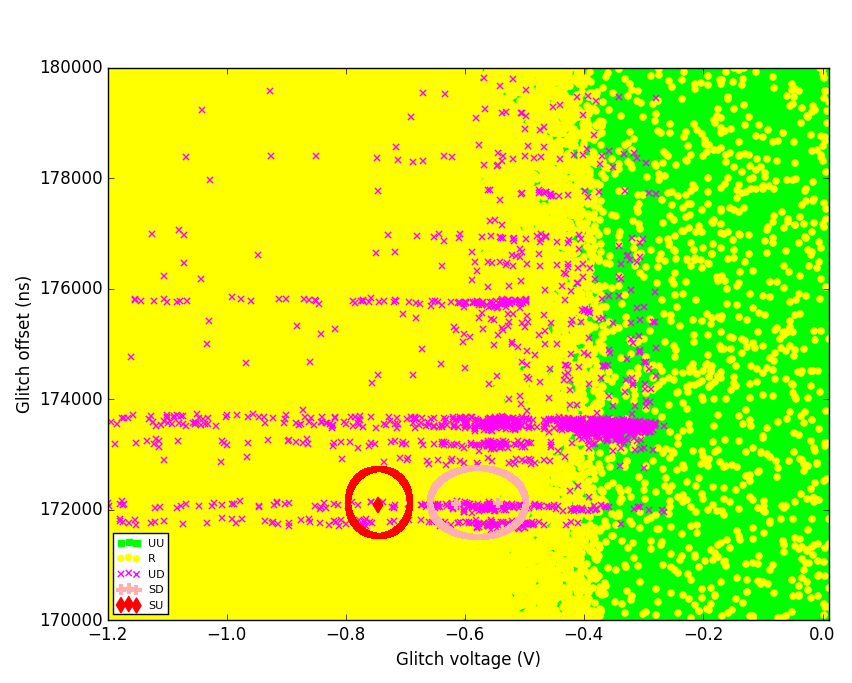
\includegraphics[width=.85\textwidth]{../../plots/newplots/ti-jtag-voltage-offset.png}
    \end{figure}
\ \\
% 260 000 measurements
\end{frame}



\begin{frame}{Characterize}{Branch experiment results summary}
    \begin{table}[H]
          \centering
          \begin{tabular}{c c c}
          \toprule
            \cellcolor{white!100} Target & Successful & Detected \\
            \midrule
            \includegraphics[width=.2\textwidth]{../../pics/tms570-cutout.png} & \multirow{ 2}{*}{60\%} & \multirow{ 2}{*}{0\%} \\ TI (power) & &\\
            \cmidrule{1-3}
            \includegraphics[width=.2\textwidth]{../../pics/spc570-cutout.png} & \multirow{ 2}{*}{58\%} & \multirow{ 2}{*}{0\%} \\ STM (EM) & &\\
          \bottomrule
          \end{tabular}
    \end{table}
    
\end{frame}

\begin{frame}{Characterize}{ Comparison of triggered measures in TI}
    % \begin{itemize}
    %     \item Comparison of triggered measures in TI
    % \end{itemize}
    
    \begin{table}[H]
          \centering
          \begin{tabular}{r r r}
          \toprule
            Successful & Detected & Other \\
            \midrule
            % Experiment 1 (ADD) & 0.7\% & 25\% & 74\% \\
            % Experiment 2 (CHECK) & 
            0.7\% & 24\% & 75\% \\
          \bottomrule
          \end{tabular}
    \end{table}

\end{frame}

\begin{frame}{Characterize}{ Comparison of triggered measures in TI}
    % \begin{itemize}
    %     \item comparison of two experiments that allow for such investigation
    % \end{itemize}
    

    \begin{table}[H]
          \centering
          \begin{tabular}{ r r r}
          \toprule
             Lockstep & RAM parity & Flash address parity \\
            \midrule
            % ADD & 92\% & 26\% & 12\% \\
            % CHECK &
             98\% & 21\% & 27\% \\
          \bottomrule
          \end{tabular}
    \end{table}

    % \begin{itemize}
    %     \item Most effective: lockstep
    % \end{itemize}
\end{frame}

\begin{frame}{JTAG}
    \begin{figure}[H]
      \centering
      \includegraphics[width=.7\textwidth]{../../pics/tms570-cutout.png}
      % \caption{\TI \unroll glitch offset vs. length}
      % \label{fig:ti-unroll-offset-length}
    \end{figure}
\end{frame}

\begin{frame}{JTAG}
    \begin{itemize}
        \item Read / write access to memory
        \item Find secret values, intellectual property
    \end{itemize}
        
    % \begin{itemize}
    % \end{itemize}
\end{frame}
    
\begin{frame}{JTAG}
    \begin{itemize}
        \item Locked, unlockable by providing password
        \item No knowledge of firmware
        \item No clear trigger signals available
        \item No register output to categorize
    \end{itemize}
\end{frame}

\begin{frame}{JTAG}
    \begin{itemize}
        \item Inject fault during boot
        \item Obtain JTAG password
    \end{itemize}
\end{frame}

\begin{frame}{JTAG}
    \begin{enumerate}
        \item Investigate normal behavior through (side) channels 
        \item Determine rough ranges of values for different parameters
        \item Determine fixed values for parameters that yield good results
    \end{enumerate}
\end{frame}


\begin{frame}{JTAG}{1. Investigate normal behavior through (side) channels }
    \begin{figure}[H]
      \centering
      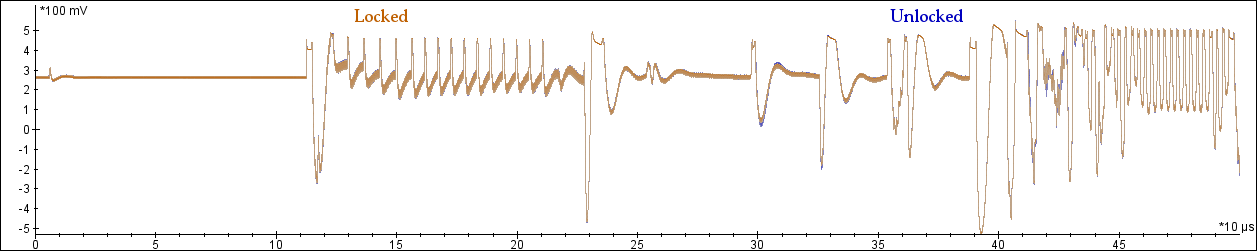
\includegraphics[width=\textwidth]{../plots/tms57-trace1.png}
    \end{figure}
\end{frame}

\begin{frame}{JTAG}{1. Investigate normal behavior through (side) channels }
    \begin{figure}[H]
      \centering
      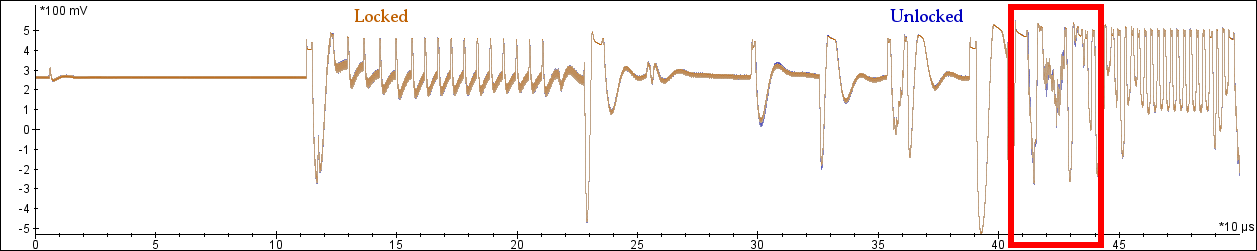
\includegraphics[width=\textwidth]{../plots/tms57-trace1-2.png}
    \end{figure}
\end{frame}

\begin{frame}{JTAG}{1. Investigate normal behavior through (side) channels }
    \begin{figure}[H]
      \centering
      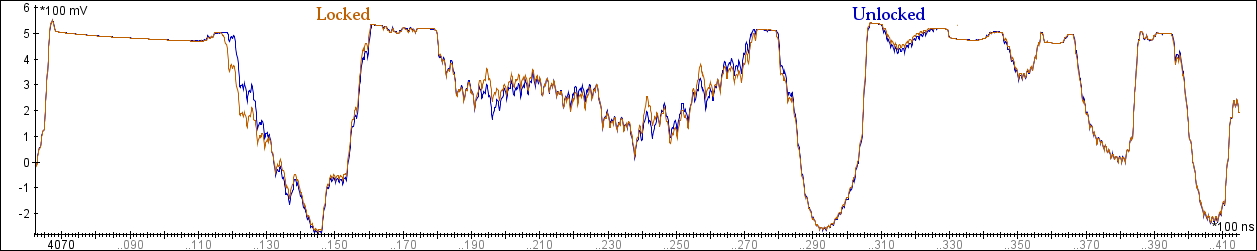
\includegraphics[width=\textwidth]{../plots/tms57-trace2.png}
    \end{figure}
\end{frame}

\begin{frame}{JTAG}{1. Investigate normal behavior through (side) channels }
    \begin{figure}[H]
      \centering
      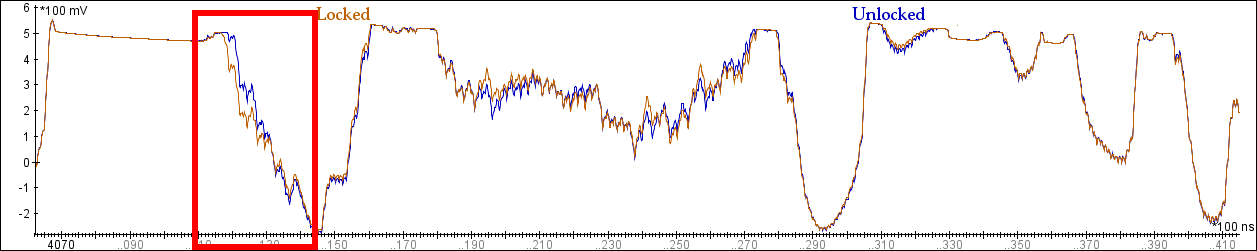
\includegraphics[width=\textwidth]{../plots/tms57-trace2-2.png}
    \end{figure}
\end{frame}

\begin{frame}{JTAG}
    \begin{table}[H]
          \centering
          \begin{tabular}{c c c}
          \toprule
            \cellcolor{white!100} Target & Successful & Detected \\
            \midrule
            \includegraphics[width=.2\textwidth]{../../pics/tms570-cutout.png} & \multirow{ 2}{*}{1.4\%} & \multirow{ 2}{*}{4.5\%} \\ TI (power) & &\\
            % \cmidrule{1-3}
            % \includegraphics[width=.2\textwidth]{../../pics/spc570-cutout.png} & \multirow{ 2}{*}{58\%} & \multirow{ 2}{*}{0\%} \\ STM (EM) & &\\
          \bottomrule
          \end{tabular}
    \end{table}
\end{frame}

\section{Conclusions\ \ }

\begin{frame}
    \tableofcontents[currentsection]
\end{frame}

\begin{frame}{Conclusions}
    \begin{itemize}
        \item These specific hardware countermeasures not  good enough for detection by themselves
        \item Of the mechanisms, lockstep most effective as countermeasure
        \item Proper mitigation requires additional measures, either additional in hardware or in software
    \end{itemize}

    \begin{table}[H]
        \centering
        \begin{tabular}{l r r}
        \toprule
        \cellcolor{white!100} & Software & Hardware \\
        \cmidrule{1-3}
        Latency         & higher           & \textbf{lower} \\
        Cost            & \textbf{lower}   & higher \\
        Fixability      & \textbf{easier}  & harder \\
        Responsibility   & implementor& silicon          \\
        \bottomrule
        \end{tabular}
  \end{table}

\end{frame}

% \begin{frame}
% \begin{table}[H]
%     \centering
%     \begin{tabular}{rccccccc}
%     \toprule
%     Assurance level &&& Low &  \multicolumn{3}{c}{$\xrightarrow{\hspace*{3cm}}$}      & High \\
%                     % &&& &&&&\\
%     Category        &&& QM  & ASIL-A & ASIL-B & ASIL-C & ASIL-D \\
%     % \cmidrule{1-6}
%     \end{tabular}
%     \caption{ASIL categories} 
%     \label{tab:ASIL}
%   \end{table}
% \end{frame}

\end{document}